\parx
Figure \ref{fig:cn_assessment} shows the Assessments window for accessing the
different built-in coding exercises for the users to try and solve. The
Assessments window can be toggled open by the keyboard shortcut \textbf{ctrl
+ shift + a}.

\begin{figure}[H]
	\centering
	\captionsetup{justification=centering}
	\captionsetup[figure]{list=yes}
	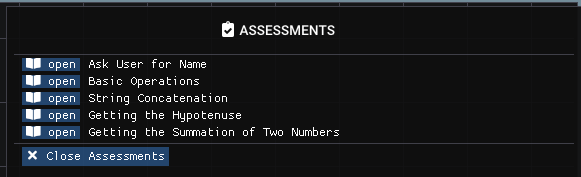
\includegraphics[width=\linewidth]{media/sc_assessments.png}
	\caption[Assessments in CodeNect]{Assessments in CodeNect}
	\label{fig:cn_assessment}
\end{figure}

\parx
Figure \ref{fig:cn_assessment_sample} shows an example coding exercise from the Assessments
window. The assessment exercise shows step-by-step general instruction for what to do
and shows the required output upon trying the assessment.

\begin{figure}[H]
	\centering
	\captionsetup{justification=centering}
	\captionsetup[figure]{list=yes}
	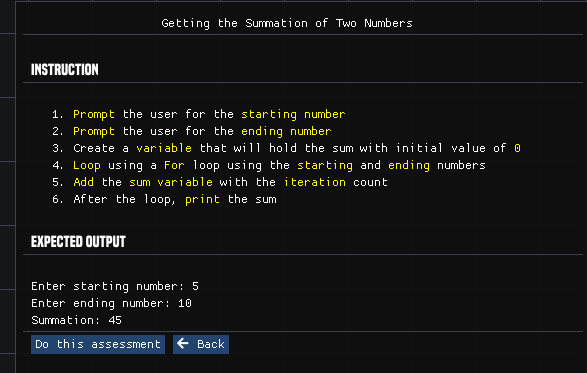
\includegraphics[width=\linewidth]{media/sc_assessments_sample.png}
	\caption[Sample Assessment in CodeNect]{Sample Assessment in CodeNect}
	\label{fig:cn_assessment_sample}
\end{figure}

\parx
Figure \ref{fig:cn_assessment_run} shows the output of a submitted visual code for
an assessment problem. The output shows a score for each line that the user got
correct. The user can also see the comparison line by line for easier checking of
the result.

\begin{figure}[H]
	\centering
	\captionsetup{justification=centering}
	\captionsetup[figure]{list=yes}
	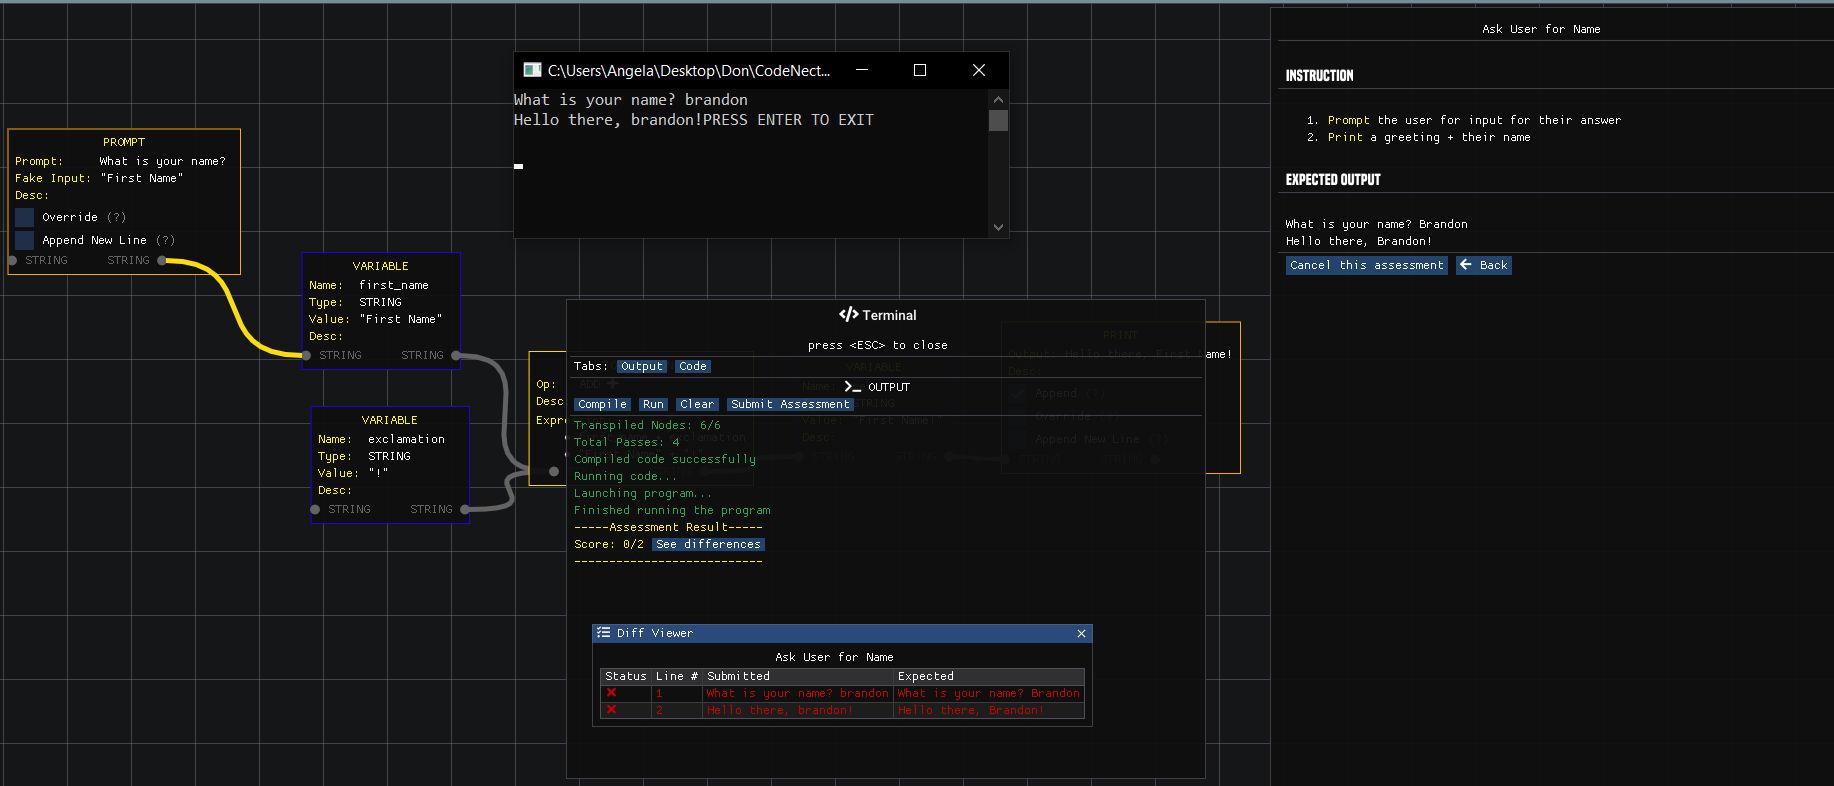
\includegraphics[width=\linewidth]{media/sc_assessments_run.png}
	\caption[Sample Assessment Output in CodeNect]{Sample Assessment Output in CodeNect}
	\label{fig:cn_assessment_run}
\end{figure}
